
\section{Results}
\label{mmf-sec:results}
This section presents the results of applying MisMatchFinder to multiple distinct datasets with different configuration. \autoref{mmf-sec:simulated data} is the evaluation of the method on simulated data, which allowed accurate and definitive insight into the sensitivity of MisMatchFinder and served as proof of concept. Then, \autoref{mmf-sec:realworld} summarises the results from multiple real world datasets, demonstrating the methods performance on real world data and the associated clinical insights.

\subsection{Simulated Data - the validation promised land}
\label{mmf-sec:simulated data}
Just like in \autoref{ch:variantcalling}, the novelty of the approach led to the issue of an absence of a gold standard dataset, with which to evaluate the performance of our new method. While there are low coverage WGS datasets of cancer patients, none of them had validated signatures associated with them. So we simulated data, to allow both optimisation of parameters of our method and granular detection of technical artefacts. 

\subsubsection{Sequencing errors filtering}
\label{mmf-sec:cleanSim}
To judge the ability of our approach to filter out sequencing errors, we first simulated ``clean`` sequencing reads with neither germline or somatic variants with the ART simulation suite \cite{Huang2011}. As current estimates of Illumina sequencing error rates were in the range of 1 in 666 to 1 in 1149 \cite{Stoler2021} which was significantly higher than even the highest tumour mutational burdens of  cancers (melanoma: 1 in 5k; tobacco smoking lung cancer: 1 in 100k) it was very important to be able to eliminate as much of the background errors as possible.

\begin{figure}[ht]
\centering
\includegraphics[width=.99\linewidth]{Figures/MisMatchFinder/mismatchrateCleanSequencing.pdf}
\caption[Mismatchrate of different filtering methods]{Mismatchrate of different filtering methods on sequencing data simulated with ART\cite{Huang2011} for both 10x and 3x coverage; Mismatches correspond to simulated sequencing errors; all: no filters, overlap: only use the overlapping parts of paired end reads with consensus building (\protect\autoref{mmf-sec:consensus}), strict OL: overlap but reads \emph{must} agree, high BQ strict OL: strict OL with high BQ in both variants; A) Absolute counts B) counts from A normalised by the number of analysed bases all: all aligned bases, other: number of bases in read overlap}\label{fig:mmf-mismatchrate}
\end{figure}

By only using high base quality mismatches, where both reads agree on the mismatch 99.98\% of all sequencing errors could be eliminated and only 1 mismatch in 10M bases would be wrongly counted as a variant (\autoref{fig:mmf-mismatchrate}). This false discovery rate was multiple orders of magnitude lower than without consensus computation and the remaining error rate was lower than most tumour mutational burden estimates \cite{Alexandrov2020,Lawrence2013a}. We therefore considered our assumption of constant and small sequencing error contribution to be correct (\autoref{mmf-sec:concept}).


\subsubsection{Spike-in signature detection}
\label{mmf-sec:simSignatures}
With the technical errors eliminated in simulated data, we used a similar method in real world data. However, to also establish a baseline for the detection limit and sensitivity of the method, we decided to first use a hybrid approach. We spiked somatic variants into genuine cfDNA low coverage WGS sequencing data of a healthy control, reducing the amount of unknown variability from other published datasets.

While it would have been possible to simulate the variants completely de novo, without any prior knowledge, we know that somatic mutations follow a certain pattern and there are mutational hotspots \cite{Chen2016,Moore2021}, so we decided to instead use the COSMIC database \cite{Tate2018,WSI2021} as the catalogue to select mutations from. This allowed us to randomly draw mutations, which occurred in a specific cancer subtype. By using COSMIC variants our simulations were less synthetic. The in-depth protocol is shown in \autoref{ch-mmfAppendix:spikein}. The downside of this method is that the spike-ins were not predominantly introduced on shorter fragments, as would be the case with real ctDNA. 

The following section discusses the results for the simulation of the very distinct SBS7a UV signature (see \autoref{fig:sig7a}) which is predominantly present in Melanoma and secondly the much flatter and more uniform SBS3 (\autoref{A:fig:sig3}), which is a sign of defective homologous recombination in breast and other cancers. 


\begin{figure}[ht]
\centering
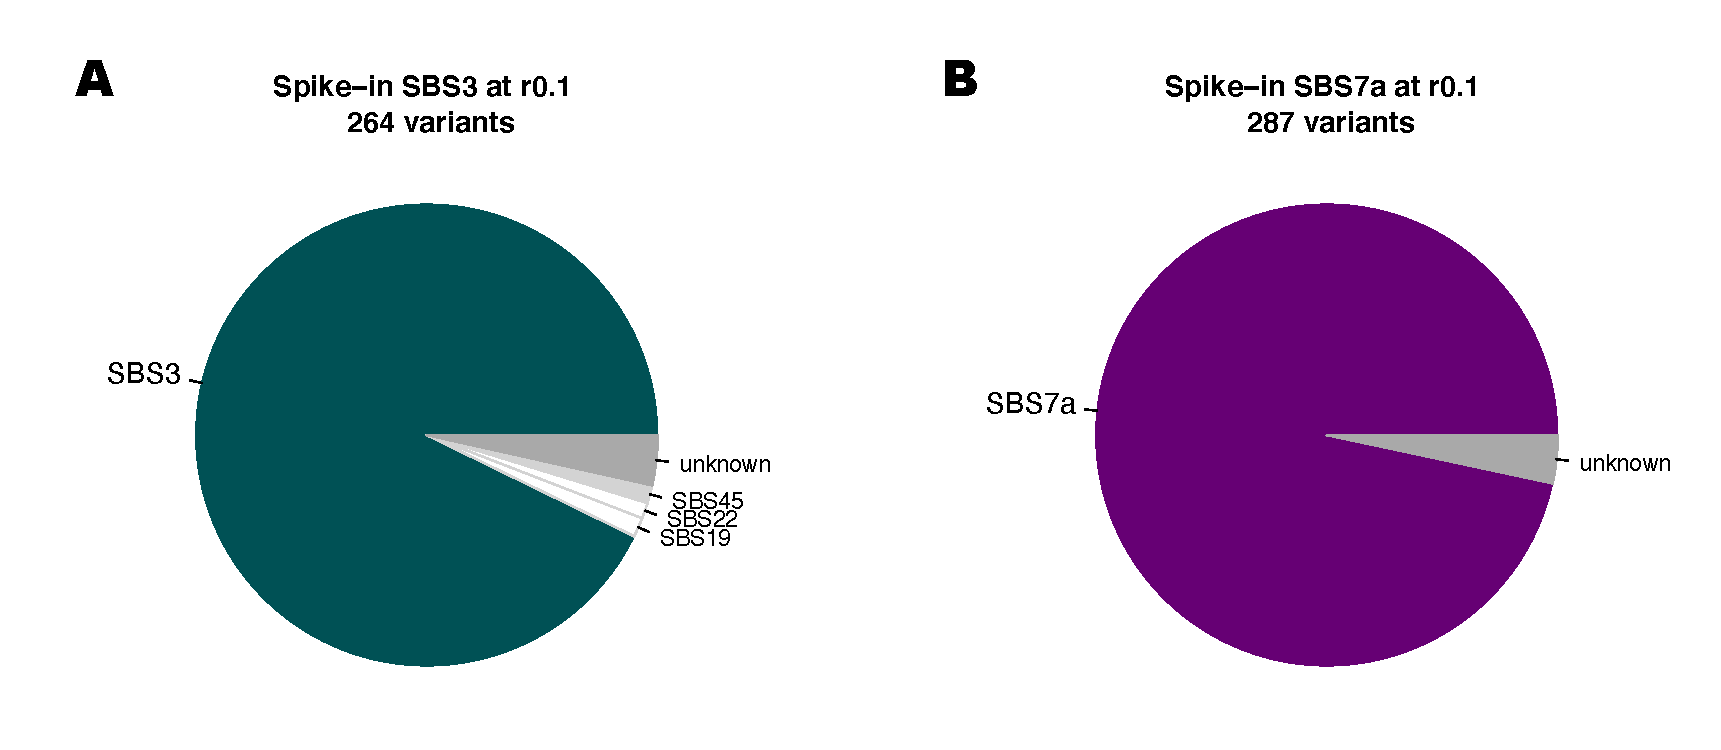
\includegraphics[width=.9\linewidth]{Figures/MisMatchFinder/spikeInSanityCheck.pdf}
\caption[Signature analysis of spike-in somatic variants]{Signature analysis results of spiked-in somatic variants; signatures with a weight less than 1\% were collated into ``unknown``; The original spike-in signature was coloured in green (SBS3) and purple (SBS7a), unrelated signatures are coloured white and signatures corresponding to sequencing artefacts are coloured in lightgrey; r0.1 corresponds to approximately 0.1 variants per mega base; Weights were generated with deconstructSigs \cite{Rosenthal2016} }\label{fig:mmf-spikeinsanity}
\end{figure}

The spike-in was done at multiple different ratios, to simulate varying tumour purities and tumour mutational burden (TMB). \autoref{fig:mmf-spikeinsanity} shows the signature analysis result of the lowest spike-in ratio ``r0.1`` which corresponded to 0.1 somatic variants per mega base and resulted in approximately 300 variants for the whole genome. As the spike-in process had to satisfy certain quality measures, not all candidate variants could be used. As such, the final simulated BAM contained 264 additional variants for the SBS3 simulation and 287 for the SBS7a equivalent. The variants corresponded to 304 and 364 ``tumour`` reads respectively within the $\approx$ 261 million reads of the simulated BAM. With increasing ratio, the spike-in signatures showed decreasing weights for other signatures, which likely got introduced due to the incomplete spike-in process (\autoref{ch-mmfAppendix:spikein}).


\begin{figure}[ht]
\centering
\includegraphics[width=.99\linewidth]{Figures/MisMatchFinder/deconstructionMethodsDifferences.pdf}
\caption[Signature weight differences for different deconvolution methods]{Signature weight differences for different deconvolution methods; Methods are the quadratic programming (QP) and iterative linea model (ILM); deconvolution was performed on the same counts generated with MisMatchFinder on 7 simulated dataset with increasing mutational burden from 5 to 100 mutations per mega base spike-in; for 0 mutations per mega base, the normal sample used for the spike-in was used}\label{fig:mmf-methodDifferences}
\end{figure}


\paragraph{Melanoma - UV exposure (SBS7a)}
\label{mmf-sec:melaSim}

With melanoma, the previously reported normal TMB ranges from 0.1 to 100 mutations per mega base \cite{Alexandrov2020}. Melanoma is usually seen as a cancer with very high mutational load, which made it the ideal target for our new mutation based tool. With only the strict overlap (\autoref{mmf-sec:consensus}) and the germline (\autoref{mmf-sec:germlinefiltering}) filtering enabled, we could see that already from r5, which represented 16899 mutated reads (of 260 Mio.), we could detect the UV signature SBS7a. While this signal would likely be too low to trust in a clinical setting, with r10, the signature weight wass already 2\% and well established. Additionally, the method was very specific on this dataset. Only SBS7a showed an increase with higher spike-in rate, with minor contributions from other other C>T heavy signatures like SBS2 and SBS30 (\Autoref{fig:mmf-methodDifferences,fig:mmf-spikeSBS7asignatures}), which partly already stemmed from the spike-in process, which was slightly enriched for SBS2 (\autoref{fig:mmf-spikeinsanity}B ``unknown``). All other signatures, which were present in the normal sample showed a decrease. This decrease was to accommodate an additional signature, as all signature weights need to sum up to 1.


\begin{figure}[ht]
\centering
\includegraphics[width=.99\linewidth]{Figures/MisMatchFinder/SBS7SpikeInSignatureDifferencesFocussed.pdf}
\caption[Signature weights differences from normal for SBS7a spike-in]{Signature weights differences from normal for SBS7a spike-in; Weights were de-constructed with QP method in MisMatchFinder and the weights assigned to the normal sample used for the spike-in were subtracted; Only Signatures with $\text{original weight}\geq 1\%$ or a minimum difference of 0.5\% are shown. The full weights can be seen in \protect\autoref{A:fig:sbs7aspikeindifferences}; r0.1 corresponded to 0.1 mutations per mega base (287 variants) and r100 was the equivalent of 100 mutations per mega base (286974 variants)}\label{fig:mmf-spikeSBS7asignatures}
\end{figure}

\paragraph{Defective homologous recombination-based DNA damage repair (SBS3)}
\label{mmf-sec:mbcSim}

Just as with the SBS7a signatures, even for the much more diffuse signature SBS3, MisMatchFinder specifically revealed the spike-in signature and did not assign the additional mismatches to any other signature. There was a small increase in SBS4 for the very low mutation rate simulations, where no SBS3 was detected. Unsurprisingly, the detection limit for SBS3 was slightly higher than for SBS7a (5 vs. 15 mutations per mega base), because of its more uniform profile. Exactly as with SBS7a, all other signatures showed a slight decrease, to accommodate the additional signature weight (\Autoref{fig:mmf-methodDifferences,fig:mmf-spikeSBS3signatures}). While the detection threshold was slightly higher than the currently assumed median TMB in breast cancer, especially triple negative breast cancer (TNBC) has shown a higher TMB, which was at comparable levels to the limit of detection we saw in this simulated dataset \cite{BarrosoSousa2020}.

\begin{figure}[ht]
\centering
\includegraphics[width=.99\linewidth]{Figures/MisMatchFinder/SBS3SpikeInSignatureDifferencesFocussed.pdf}
\caption[Signature weights differences from normal for SBS3 spike-in]{Signature weights differences from normal for SBS3 spike-in; Weights were deconstructed with QP method in MisMatchFinder and the weights assigned to the normal sample used for the spike-in were substracted; Only Signatures with $\text{original weight}\geq 1\%$ or a minimum difference of 0.5\% are shown. The full weights can be seen in \protect\autoref{A:fig:sbs3spikeindifferences}; r0.1 corresponds to 0.1 mutations per megabase (264 variants) and r100 is the equivalent of 100 mutations per megabase (285367 variants)}\label{fig:mmf-spikeSBS3signatures}
\end{figure}

\subsubsection{Germline filtering}
\label{mmf-sec:germlinefiltering}
In order to ensure our assumptions also hold true in real patient data, we evaluated the effect of removing germline variants from the analysis. We utilised the same simulated samples from \autoref{mmf-sec:simSignatures}, where the reads were original cfDNA sequencing reads from a healthy person. These reads had a known natural background germline variant profile as any arbitrary sample would.

\begin{figure}[ht]
\centering
\includegraphics[width=.99\linewidth]{Figures/MisMatchFinder/noGermlineFilterAnalysis.pdf}
\caption[Signature analysis without germline variant filtering]{Signature analysis without germline variant filtering; Weights were deconstructed with QP method in MisMatchFinder, but in contrast to \protect\autoref{fig:mmf-methodDifferences}, the filter removing all known germline variants was disabled}\label{fig:mmf-noGermlineFilterAnalysis}
\end{figure}

In stark contrast to the previous analysis (\autoref{fig:mmf-methodDifferences}), when retaining mismatches in known germline variant sites, the sensitivity of the method reduced significantly. Only for the SBS7a spike-in at the very highest mutation frequency (100 mutations per mega base) was a signal detected. This signal was still weaker than what was previously found with just 10 mutations per mega base. Unsurprisingly SBS3 performed worse, just as before, and no signal was detected at any frequency (\autoref{fig:mmf-noGermlineFilterAnalysis}).

This extreme change was caused by the much higher number of mismatches which were used in the analysis ($\approx 1.8$ Mio without germline filter and $\approx 130$K with germline filter).
This increase in mismatches in the analysis diluted the spike-in variants. \autoref{fig:mmf-percentIncrease} showed that without the germline filter the additional found mismatches never exceeded 5\% of all mismatches, which seemed to be the detection threshold for SBS7a. With germline filtering this threshold corresponded perfectly with the increase of SBS7a weight in those samples (\autoref{fig:mmf-methodDifferences}).

\begin{figure}[ht]
\centering
\includegraphics[width=.99\linewidth]{Figures/MisMatchFinder/spikeInPercentage.pdf}
\caption[Percent increase of mismatches in analysis with and without germline filter]{Percent increase of mismatches in analysis with and without germline filter; Values are normalised to the number of mismatches found in the normal sample (depicted as \num{0} mutations per mega base); dotted grey line shows the maximum increase in the left panel (without germline filter)}\label{fig:mmf-percentIncrease}
\end{figure}

While we had already established that the spike-in variants could not  be detected when retaining germline variant sites, the computed signature weights in the normal sample were vastly different as well. Without the germline filter, the most prevalent signatures were SBS1 and SBS5 which are thought to be molecular clock like signatures, related to the age of the individual \cite{Alexandrov2020}. In the germline filtered analysis the most prevalent signatures were SBS4 (tobacco smoking), SBS12 (unknown) and SBS46 (sequencing artefact). In general it seemed like the germline filter removed predominantly SBS1 and SBS5, while most other signatures remained the same (\autoref{fig:mmf-noGermlinePie}).

As the sample was acquired through a healthy donor blood bank, we had no way to verify if the individual was a smoker.

\begin{figure}[ht]
\centering
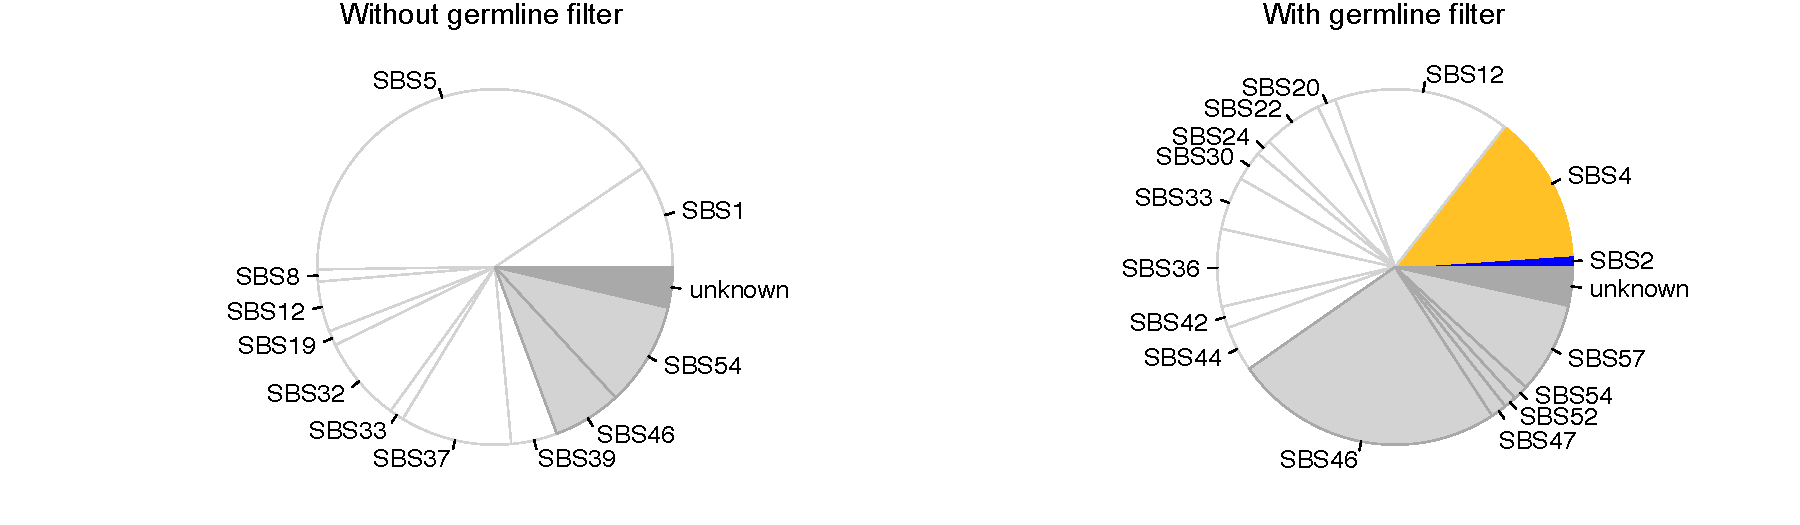
\includegraphics[width=.99\linewidth]{Figures/MisMatchFinder/noGermlineFilterSignaturesPieChart.pdf}
\caption[Signature weights of the normal sample with and without germline filter]{Signature weights of the normal sample with and without germline filter; MisMatchFinder derived signature weights with and without germline filter; weights below 1\% contribution are accumulated in ``unknown`` (darkgrey), lightgrey signatures show sequencing artefact signatures, yellow shows smoking related signatures and blue depicts APOBEC signatures}\label{fig:mmf-noGermlinePie}
\end{figure}
 
This convinced us that germline filtering, additionally to the consensus overlap analysis, was fundamentally important for the method to recover signal. In the following sections, unless further specified, the germline filter was enabled for all analysis.


\subsection{Real world data - analysis of patient data}
\label{mmf-sec:realworld}

While simulated data is perfect to ensure the method performs as expected in edge cases and to estimate detection limits, only real world data allows the final examination to understand if the model used for analysis can mirror biological concepts. To show our new method is usable for a variety of datasets, we used a mixture of different cancer types with different library preparation. In \autoref{mmf-sec:healthy} we focused on the analysis of 60  healthy individuals. We generated a background noise model and excluded aging as one of the sources of variation from our data. Then we analysed two metastatic breast cancer patients with BRCA1 positive disease, comparing matched tumour-normal sequencing with MisMatchFinder. This dataset allowed us to evaluate how efficient germline filtering was (\autoref{mmf-sec:germlineArtifacts}) and how accurate and sensitive our method was when compared to the current gold standard of tumour-normal tissue analysis (\autoref{mmf-sec:matchedMBCB}).
A second dataset containing samples of two cfDNA time points and corresponding tissue from a patient with metastatic melanoma allowed us to validate performance of MisMatchFinder in a different cancer context (\autoref{mmf-sec:melpatients}). Lastly we analysed a dataset of 79 tumour only cfDNA samples both melanoma (40) and breast cancer (39) patients to show the potential clinical application of MisMatchFinder (\autoref{mmf-sec:tumourDetection}). The mean tumour purity assigned to each sample by ichorCNA was 16.2\% (min: 0.3\% max: 71.5\% sd: 17.0\%) displaying a clinically expected range of high and low ctDNA fractions. The mean age of patients was 53.4 (min: 34 max: 74) for the breast cancer patients and 60.2 (min: 34 max: 81) for the melanoma patients which is very closely age matched to our healthy samples (\autoref{mmf-sec:healthy}).

In the following section, we showed that MisMatchFinder exhibits barely any technical bias.

\subsubsection{Bias detection}
\label{mmf-sec:healthyBias}
A dataset with healthy samples is key to detect biases, because any variability that cannot be accounted to either age or gender is unwanted and will affect the cancer samples in the same way. We expected an increased mismatch rate in the older individuals do to the accumulation of somatic mutations due to ``clock like signatures`` \cite{Abascal2021}. In contrast, tumour samples should be biased based on tumour purity, as higher amount of tumour reads would result in a higher amount of mismatches from somatic mutations.
To verify that our assumptions were correct, we performed a principle component analysis (PCA) of the raw tri-nucleotide mismatch count numbers, of all 79 tumour only and 60 healthy samples, which MisMatchFinder can report alongside the weights of signatures.

% latex is dumb with this figure, i want it right HERE
\begin{figure}[htp]
\centering
\includegraphics[width=.99\linewidth]{Figures/MisMatchFinder/countPCAsPC1vsPC2.pdf}
\caption[PCA of tri-nucleotide mismatch counts of real world data (PC1 and PC2)]{PCA (PC1 and PC2) of tri-nucleotide mismatch counts of healthy donor and tumour samples (melanoma and metastatic breast cancer) of varying purity; PCA was conducted on scaled and centered data}\label{fig:mmf-pca1v2}
\end{figure}


Neither age, nor sex of the sample seemed to have any influence on the mismatches of the sample \autoref{fig:mmf-pca1v2}A,~B. In contrast, there appeared to be a batch effect with regards to the used flowcell on the sequencer and library preparation (\autoref{fig:mmf-pca1v2}C,~D). As these two are strongly intertwined, it was not possible to differentiate the two effects, however the flowcell bias was evident across multiple library preparations and therefore more likely to be the source of the bias. Flowcell 1 contained samples from both \lq g\rq\ and \lq h\rq\ and  flowcell 3 both \lq a\rq\ and \lq d\rq, suggesting that the flowcell had more influence than the preparation. This is consistent with recent literature, which suggests, that there are more and less error prone flow cells \cite{Stoler2021}.

While there was a slight bias towards higher PC1 values for higher DNA input samples, which might be due to a higher library complexity when sequencing, it was minor and the same bias exists for every other method using de-duplicated sequencing data as it might have an effect on the non-redundant data available (\autoref{fig:mmf-pca1v2}E). Similarly, the very low coverage samples were at the very left of PC1, but there was a substantial spread along the axis for the higher coverage samples as well (\autoref{fig:mmf-pca1v2}F). 

As expected from the model and the biology, there was a trend of separation for both tumour type and tumour purity, with the higher purity samples oriented toward the top right and the healthy and lower purity samples at the left (\autoref{fig:mmf-pca1v2}G,~H).

These tendencies can also be observed when looking at PC2 and PC3 (\autoref{A:fig:mmf-pca2v3}). PC3 still accounts for $\approx \text{9\%}$ of the observed variability and PC6 is the first component with an variance value smaller than 1 suggesting that only the first five components should be retained for further analysis (explaining a cumulative 97.3\% of the variance). However, as we use the counts for signature deconstruction the PCA analysis only served as a quality control.


\subsubsection{Healthy cohort}
\label{mmf-sec:healthy}

We sequenced the 60 healthy samples, from varying age groups (range: \num{24}~yrs.-\num{70}~yrs. median: \num{48.5}~yrs.) with 24 males and 36 females, in the exact same way as the tumour only samples for breast cancer and melanoma to an effective average coverage of 8x WGS, with mixed healthy samples and cancer samples on sequencing flow cells to account for and minimise batch effects.

With recent literature indicating a linear relationship of aging and somatic mutations \cite{Martincorena2018,Abascal2021,Cagan2022}, we were interested if the MisMatchFinder method could identify the accumulation of  somatic mutations with age. While the samples between 30 and 59 showed the expected linear increase in mean mismatch rate, both the 20-29 and 60-69 year old samples showed the inverse trend, where young individuals exhibited a higher mismatch rate than older. This discrepancy could have been rooted in the germline filtering step as shown in \autoref{mmf-sec:germlineArtifacts}, or it may have been a sign of loss of heterogeneity in the hematopoiesis as shown in aging mice \cite{Ganuza2019}. Lastly, with only 40 healthy samples, we might not have had enough representation in each age group to detect subtle changes.Whatever the source, MisMatchFinder was not able to infer the age of a sample with the default settings in this dataset.

\begin{figure}[ht]
\centering
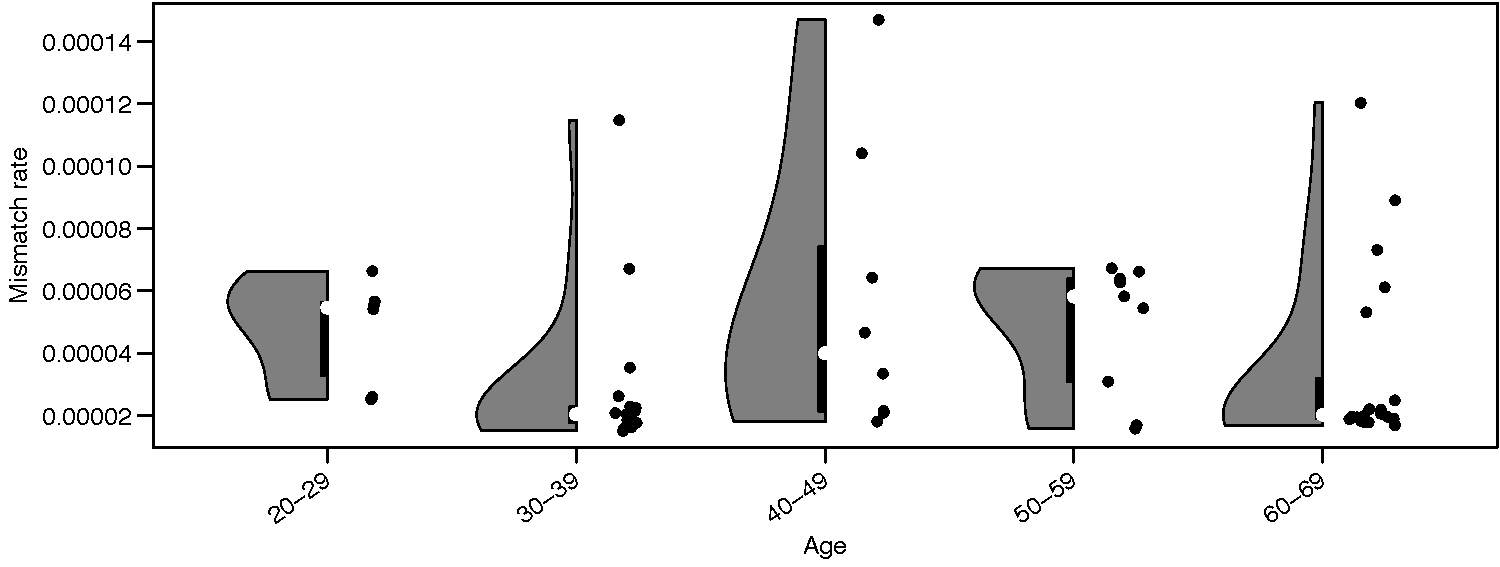
\includegraphics[width=.99\linewidth]{Figures/MisMatchFinder/MisMatchRateByAge.pdf}
\caption[Mismatchrates of healthy samples by age]{Mismatchrates of healthy samples by age: distribution of sample is shown as violin plots on the left hand of each group, with a boxplot and the mean indicated as a black box and a white dot respectively; Observed values were displayed as black dots on the right hand of each group}\label{fig:mmf-mmrByAge}
\end{figure}


\paragraph{Black list generation}
\label{mmf-sec:healthyBlacklist}
With the strong effect filtering of both technical errors (\autoref{mmf-sec:cleanSim}) and germline variants (\autoref{mmf-sec:germlinefiltering})  as background noise had on our method, we hypothesised that a blacklist of mismatches found in our healthy individuals would help us further cut down on unwanted background signal and refine the somatic mismatch calls. We therefore ran MisMatchFinder with significantly relaxed quality cut-offs to capture as much variation as possible. This included a reduction in mapping quality and base quality as well as not restricting the analysis to the highly accurate overlap part of the paired end reads. However we still restricted the analysis to the same highly mappable areas of the genome the same as for the tumour analysis as well as filtering already known germline variants for a better estimation of the impact of this filter step.

The site files generated through MisMatchFinder were then concatenated and aggregated to multiple blacklists with cut-offs of a variant present in at least 3, 5 or 10 times. The code used for the post processing of MisMatchFinder site files can be found in \autoref{lst-mmf:blacklist}.


\begin{figure}[ht]
\centering
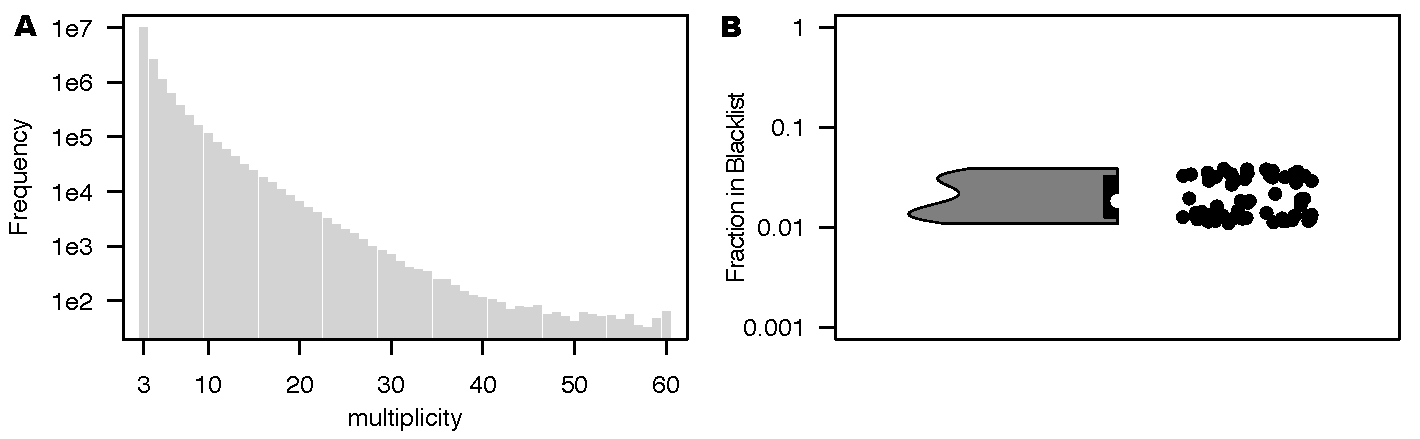
\includegraphics[width=.99\linewidth]{Figures/MisMatchFinder/mmfBlackListStats.pdf}
\caption[Blacklisted mismatches from healthy individuals]{Blacklisted mismatches from healthy individuals: A) Histogram of frequency of mismatches found by at least n samples (multiplicity) B) Percentage of mismatches in healthy samples found in blacklist of mismatches found in at least three healthy samples; violin plot with median as white dot (left) and real values (right)}\label{fig:mmf-BlackListStats}
\end{figure}

While there was a substantial number of shared variants in the reduced parameter analysis out of the $\approx 15$ million mismatches, only 3413 were in more than 50\% of all samples (\autoref{fig:mmf-BlackListStats}A), and the blacklist filtering  did not lead to a performance boost. When we used the default settings for the healthy samples and used the generated blacklist as a filter on average only 2\% of mismatches were removed by the blacklist assignment (min: 1\%, max: 3\%) when at least three samples showed the mismatch (\autoref{fig:mmf-BlackListStats}B). Utilising the ten sample blacklist, the mean filtering amount dropped to 0.1\% of mismatches of the sample (min: 0.04\% max: 0.3\%). We therefore concluded that the blacklist filtering step has no additional benefit and it was not included in the default analysis of MisMatchFinder. 

\subsubsection{\textit{BRCA1} mutation positive breast cancer patient samples}
\label{mmf-sec:brcapatients}
The first dataset of cancer patients involved two BRCA1 mutation positive females. The data contained matched tumour, germline and cfDNA sequencing with high depth ($\approx 80x$) WGS for all samples. With the matched normal, we used the current standard protocol of somatic mutational pattern analysis (\autoref{mmf-sec:signatureanalysis}) and compared it with our new method (\autoref{mmf-sec:matchedMBCB}). 

As the sequencing data had a much higher depth than what is used in standard clinical practice for plasma sequencing, we down-sampled the data to 8x coverage for MismtachFinder analysis, bringing it in line with the simulated data. By using several different seeds for the sampling, we generated pseudo technical replicates of the sequencing (\autoref{ch-mmfAppendix:subsampling}), which in term gave an approximation of the stability of the results of MisMatchFinder.


\paragraph{Germline artifacts}
\label{mmf-sec:germlineArtifacts}
As discussed above, the germline filter step is vital to boost the signal of somatic variants (\autoref{mmf-sec:germline}). We were interested in how many germline variants were not filtered out with our filtering step and were still contributing to background noise. The high depth matched healthy WGS samples of the breast cancer patients was used for this analysis. We called germline variants on the matched normal using Strelka2 and compared the called variants with the sites reported by MisMatchFinder as somatic (retained after germline filtering) on the sub-sampled data. All variants with any quality filter assigned by Strelka2 were considered for this analysis, such that possible clonal hematopoiesis (CH) variants were still considered. \autoref{tab:mmf-germlineArtifacts} showed that on average 2100 germline variants were not filtered out per run. However, this only equated to 0.9\% for patient 1 (MBCB196) and 1.5\% for patient 2 (MBCB298) of all sites found to be mutated. While the exact numbers of any arbitrary sample will depend on the strictness of the parameters of the analysis as well as the mutation rate of the sample, with default parameters a similar result should be expected with other samples, suggesting the germline filter was removing virtually all mismatches caused by germline variants.

The germline variant removal was therefore very effective filtering the 3.75 (MBCB196) and 3.76 (MBCB298) million germline SNPs called by Strelka2 to less than 0.05\% of the original number. As the genetic background in gnomAD is not balanced and shows a lack of non-european ancestry data \cite{Tiao2020}, this filtering could become less effective when analysing samples from indigenous or otherwise genetically less characterised patients, as their germline variants might not be comprehensively represented.

Nevertheless, this result combined with the effective filtering of technical errors (\autoref{mmf-sec:cleanSim}) suggested, that nearly all of the remaining sites were somatic mutations of either the healthy tissue or the cancer cells.

\begin{table}
\caption[Germline variants retained after germline filtering]{Germline variants retained after germline filtering with MisMatchFinder analysis; Default parameters were used when running MisMatchFinder with gnomAD zarr for filtering. seed column showed the seed used to subsample the high depth sequencing BAM, ``mismatch sites`` column contains number of sites found to be changed, ``germline sites`` contains the number of sites also found with germline variant calling, fraction shows fraction of column 4 and 3}\label{tab:mmf-germlineArtifacts}
\centering
\begin{tabular}{|c|c|c|c|c|}
\toprule
\hline
\textbf{Patient ID} & \textbf{seed} & \textbf{mismatch sites} & \textbf{germline sites} & \textbf{fraction} \\
\hline
 & \num{1007} & \num{216950} &  \num{2107} & \num{0.0097}\\ 
 & \num{1234} & \num{217145} &  \num{2073} & \num{0.0095}\\ 
 & \num{1337} & \num{216823} &  \num{2080} & \num{0.0096}\\ 
 & \num{1717} & \num{217593} &  \num{2089} & \num{0.0096}\\ 
 & \num{2358} & \num{217317} &  \num{2097} & \num{0.0096}\\ 
 & \num{3311} & \num{217219} &  \num{2046} & \num{0.0094}\\ 
 & \num{5229} & \num{216876} &  \num{2062} & \num{0.0095}\\ 
 & \num{6060} & \num{217388} &  \num{2080} & \num{0.0096}\\ 
\multirow{-9}{*}{MBCB196} & \num{9876} & \num{217656} &  \num{2008} & \num{0.0092}\\ 
\hline
 & \num{1756} & \num{148495} &  \num{2168} & \num{0.0146}\\ 
 & \num{3599} & \num{149901} &  \num{2224} & \num{0.0148}\\ 
 & \num{4117} & \num{149382} &  \num{2277} & \num{0.0152}\\ 
 & \num{4306} & \num{149549} &  \num{2248} & \num{0.0150}\\ 
 & \num{4359} & \num{149805} &  \num{2205} & \num{0.0147}\\ 
 & \num{5788} & \num{150103} &  \num{2241} & \num{0.0149}\\ 
 & \num{5887} & \num{150099} &  \num{2287} & \num{0.0152}\\ 
 & \num{8387} & \num{149533} &  \num{2248} & \num{0.0150}\\ 
\multirow{-9}{*}{MBCB298} & \num{9754} & \num{149547} &  \num{2229} & \num{0.0149}\\
\hline
\bottomrule
\end{tabular}
\end{table}


Additionally, we were interested to see if the filtering did remove true somatic signal, by removing somatic variants which mirrored a known germline variant. We therefore annotated high confidence variants called with Strelka2 in both the patient tumour tissue and cfDNA samples with a germline flag when that variant was previously found in gnomAD. Surprisingly we found that $\approx 50\%$ of somatic variants found in any sample were also found in gnomAD. To ensure these samples were not outliers, we also analysed the tissue samples from \autoref{ch:cascade} and saw that all samples had half of the somatic variants called already present in gnomAD (\autoref{fig:mmf-germlineStatus}A). While gnomAD is known to contain potential somatic contamination, these overlaps were most likely due to error prone sites in the genome and the higher rate of deaminations and transitions over transversions \cite{Meyerson2020}. To ensure our filtering did not skew the results we performed signature deconvolution on the somatic variants of a sample, which were not found in gnomAD and variants which were found in gnomAD. While there were minor signatures, which were clinically relevant (SBS13 and SBS87) in the ``germline`` partition, the majority of signatures were identified using variants not contained in gnomAD. Specifically SBS13's contribution was larger in the non-germline selection even though it was found in both analyses (\autoref{fig:mmf-germlineStatus}B vs C, \autoref{A:fig:signaturesGermlineSplit}).

\begin{figure}[ht]
\centering
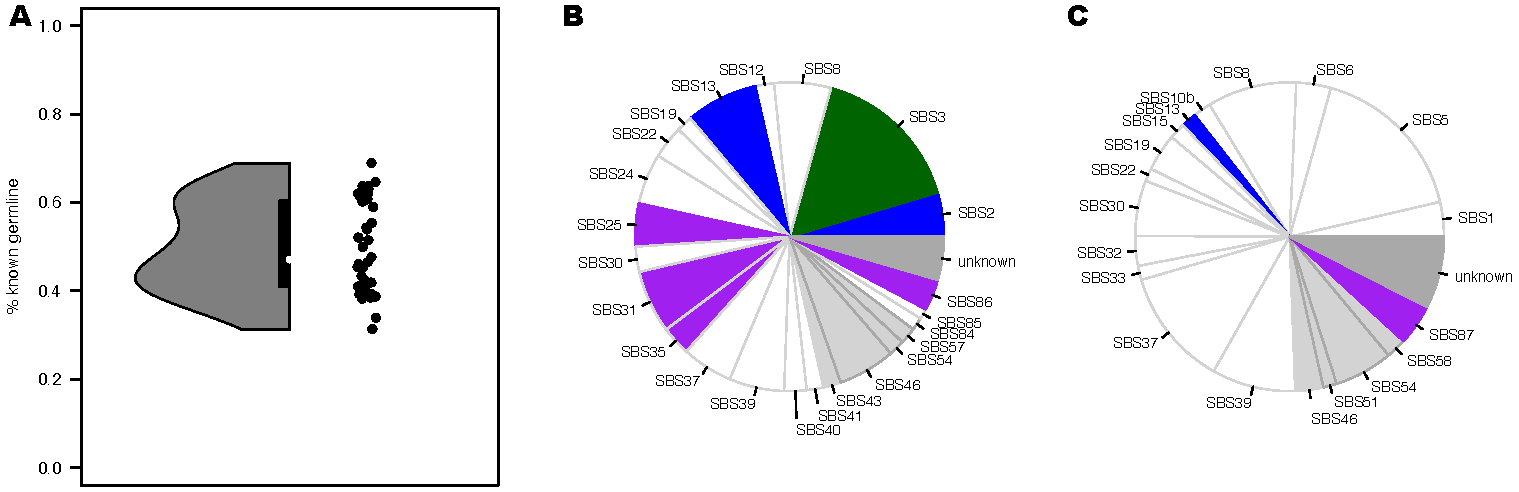
\includegraphics[width=.99\linewidth]{Figures/MisMatchFinder/somaticVarsInGermlineSites.pdf}
\caption[Somatic variants found in germline sites]{Analysis of somatic variants with respect to germline database gnomAD: A) percentage of somatic variants called with Strelka2 found also in gnomAD; Violin plot with median as white dot (left) and values (right)  B) signature analysis of variants not found in gnomAD for sample MBCB196 cfDNA c) signature analysis of variants also found in gnomAD for sample MBCB196 cfDNA; Colours show cancer associated signatures: blue (APOBEC), red (UV exposure), orange (tobacco), purple (chemotherapy), light grey (sequencing artefacts), dark grey (everything below 1\% weight)}\label{fig:mmf-germlineStatus}
\end{figure}
  


In summary, the germline filtering was a very powerful step, which boosted the performance of our signature detection method significantly with minimal signal deterioration. The high overlap of germline database variants and somatic variants poses a challenge for perfect concordance between our method and the current gold standard and would be an ideal area for further optimisation especially if ageing signatures like SBS1 and SBS5, which are caused by deamination, are  of interest. These  variants will be predominantly removed and were the most likely reason for the absence of ageing signatures seen on healthy individuals (\autoref{mmf-sec:healthyBias}). A potential solution would be to incorporate a machine learning model to distinguish germline from somatic variants \cite{Spinella2016,Sahraeian2022}.

\paragraph{Matched tissue and cfDNA WGS samples}
\label{mmf-sec:matchedMBCB}

\begin{figure}[ht]
\centering
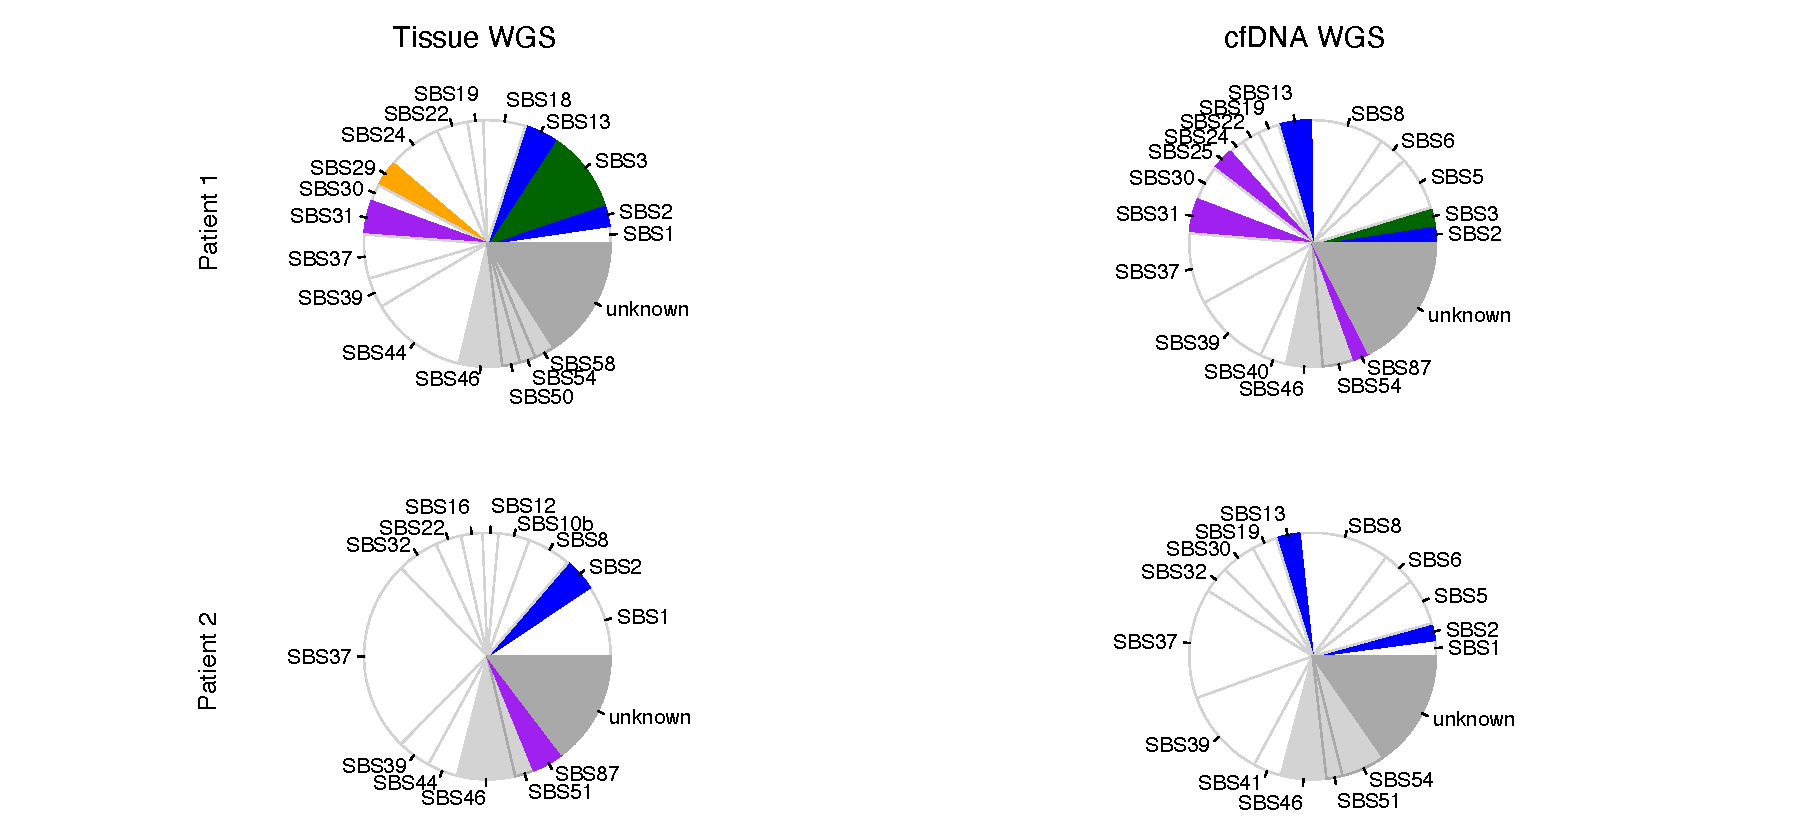
\includegraphics[width=.99\linewidth]{Figures/MisMatchFinder/mbcbWGSsignatures.pdf}
\caption[Signature weights for the WGS of two BRCA1 mutation positive breast cancer patients]{Signature weights for the WGS of two BRCA1 mutation positive breast cancer patients: Colours show cancer associated signatures: blue (APOBEC), red (UV exposure), orange (tobacco), purple (chemotherapy), light grey (sequencing artefacts), dark grey (everything below 1\% weight)}\label{fig:mmf-mbcbWGSsigPie}
\end{figure}
 
The matched tissue-normal WGS for the two metastatic breast cancer patients allowed a concordance analysis with a known true signature. We called variants with Strelka2 and performed default signature deconvolution with sigminer to obtain weights using default parameters for the GRCh38 genome build and QP deconstruction method  \cite{Wang2021}. Due to their known germline BRCA1 mutations we expected a contribution of SBS3. Both the tissue and the ctDNA samples of patient MBCB196 show a greater than 3\% SBS3 as expected, however neither samples for MBCB298 showed SBS3 (\autoref{fig:mmf-mbcbWGSsigPie}).
 
\begin{figure}[hb]
\centering
\includegraphics[width=.99\linewidth]{Figures/MisMatchFinder/brca1BarPlots.pdf}
\caption[Signature weights for subsampled BRCA1 positive patients]{Signature weights for subsampled BRCA1 positive patients: each quadrant represents one high depth WGS sample downsampled to 8x with different seed (x-axis) signature weights per downsampling were shown in the columns in each quadrant. Colours represent clinically relevant signatures: blue (APOBEC), green (HRD), red (UV radiation); light grey and white show sequencing artefact and signatures of unknown significance respectively. Only signatures considered to be active (\autoref{mmf-sec:sigdetection}) were displayed}\label{fig:mmf-mbcbBarPlot}
\end{figure}

When applying the default parameter MisMatchFinder analysis to the downsampled WGS, we observed consistent results with any seed, suggesting that the signal was present in all reads and subsampling did not skew the results. Secondly, the expected SBS3 signature was found at $\approx 18\%$ (min: 14\% max: 21\%) in the tissue and $\approx 24\%$ (min: 20\% max: 26\%) in the cfDNA, recapitulating the results from the standard analysis (\autoref{mmf-sec:sigdetection}). The chemotherapy related signatures SBS25, SBS31, and SBS87 seen in both MBCB196 and MBCB298, were not reported by MisMatchFinder. This could have been caused by the germline filtering step, however these signatures were not clinically actionable and expected after chemotherapy treatment so their exclusion was not of major concern.

Surprisingly, even though the APOBEC signatures SBS2 and SBS13 were observed in the normal signature deconvolution of patient 1 and 2, MisMatchFinder only found very low levels of SBS13 contribution in the cfDNA sample (mean: 0.4\% (min: 0.1\% max: 0.7\%) and no contribution in the tissue samples. However, MisMatchFinder was able to detect a high prevalence of SBS2 in both tissue (mean:~12\% min:~11\% max:~12\%) and cfDNA (mean:~69\% min:~65\% max~74\%) samples of MBCB298, indicating that MisMatchFinder was capable of detecting APOBEC signatures. 

Importantly, even thought the WGS analysis with sigminer did not result in a SBS3 positive deconvolution, MisMatchFinder was able to recover the expected signature in the tissue samples (mean:~28\%, min:~27\%, max:~29\%). As the tissue sample in this case was a FFPE sample, with a much higher number of somatic variants called and very low tumour purity ($\leq 13\%$) the standard analysis could have been overwhelmed with FFPE artefacts, which were successfully filtered out using MisMatchFinder. Interestingly, the cfDNA sample did not show any SBS3, but extensively high APOBEC activity. The absence of SBS3 could potentially be explained by reversion mutations in the cancer reenabling BRCA1/2 \cite{Lin2018a}, while the high APOBEC activity has been shown in some breast cancer types with Kataegis \cite{Alexandrov2020,Rebhandl2015}. Both the tissue samples of MBCB196 and the cfDNA sample of MBCB298 showed activity of UV signatures SBS38 and SBS7b respectively. While it is unlikely that these were caused by UV exposure, the APOBEC deamination signature has similarities to UV exposure. We therefore thought the UV signatures may have represented a leaky APOBEC signature rather than genuine UV exposure.

While MisMatchFinder did not detect the expected SBS3 signature in all samples, we could show a high concordance with the current gold standard analysis and MisMatchFinder revealed clinically relevant signatures SBS2 and SBS3. 

\subsubsection{Melanoma patient samples}
\label{mmf-sec:melpatients}

For melanoma real world data, we analysed samples from a single melanoma patient containing tumour-normal matched tissue WES with two additional longitudinal time points of cfDNA sequenced both through WES and lcWGS. This allowed us to compare the current standard signature analysis for both time points with our novel low coverage method that MisMatchFinder was developed for.

With the help of the WES of both the tissue and the cfDNA samples, we established the gold standard to compare the MisMatchFinder result to.  Strelka2 was used to call somatic variants and the high confidence somatic SNPs were used to generate signature weights with sigminer.

As expected from a skin melanoma, the tissue as well as both WES cfDNA samples revealed a high contribution of SBS7a and SBS7b, with approximately 50\%  of all somatic variants associated with these two signatures in the tissue and time point 1 and 27\% in time point 2. While several other signatures were found to be present in all samples, none of them had clinical relevance (\autoref{fig:mmf-melaWESsigPie}).

\begin{figure}[ht]
\centering
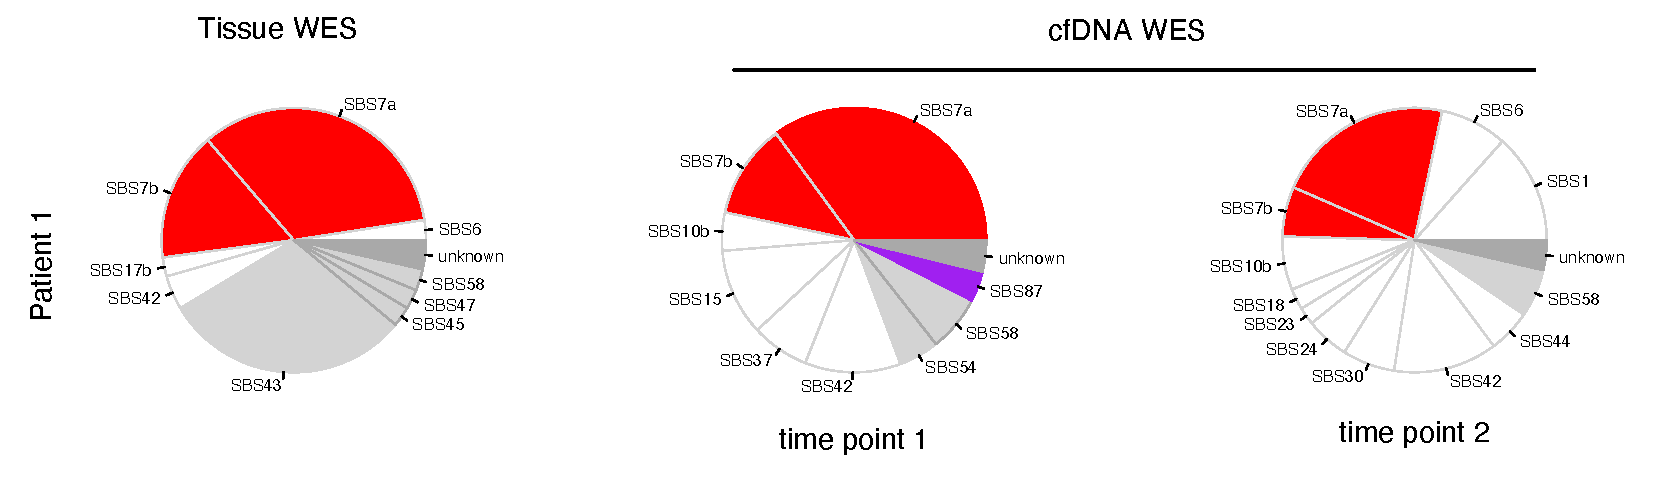
\includegraphics[width=.99\linewidth]{Figures/MisMatchFinder/melanomaWESsignatures.pdf}
\caption[Signature weights for the WES of two melanoma patients]{Signature weights for the WES of two melanoma patients; First column shows the results for the tissue baseline and middle and right column show the cfDNA; Colours show cancer associated signatures: blue (APOBEC), red (UV exposure), orange (tobacco), purple (chemotherapy), light grey (sequencing artefacts), dark grey (everything below 1\% weight)}\label{fig:mmf-melaWESsigPie}
\end{figure}
 
This high exposure of SBS7a and SBS7b was highly concordant with our analysis of the lcWGS sample of time point 1, where more than 50\% of all somatic mismatches signatures, which were called active (\autoref{mmf-sec:sigdetection}), were attributed to SBS7a and SBS7b. While the proportion of SBS7a to SBS7b was different between the WES result and the lcWGS, the weights for those signatures were very similar. Time point 2 on the other hand showed less agreement between WES (sigminer) and lcWGS (MisMatchFinder). While SBS7b was still detected at similar levels between both methods, MisMatchFinder failed to detect SBS7a, which was the highest contributing signature at time point 2 using the somatic variants from WES. Additionally both lcWGS samples show a high prevalence of SBS3, which was not detected in the WES. While SBS3 is usually accredited to \textit{BRCA1/2} positive breast cancers, there have been reports of homology repair deficiency in melanomas. These mismatches might have been caused by subclonal variants, which are below detection threshold for conventional variant calling (\Autoref{fig:mmf-melaWESsigPie,fig:mmf-melaMMFsigPie}).

\begin{figure}[ht]
\centering
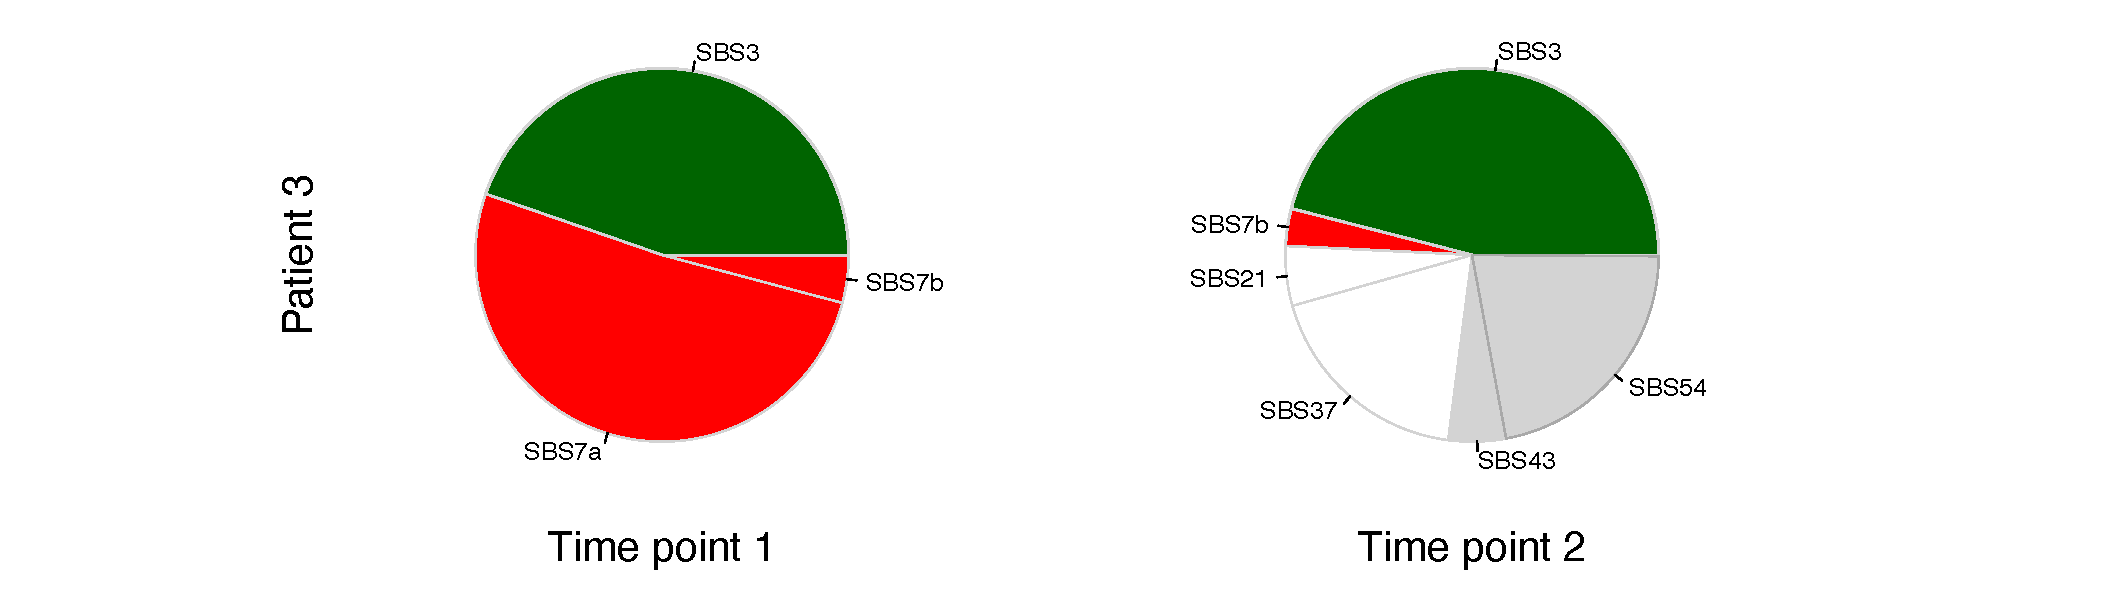
\includegraphics[width=.99\linewidth]{Figures/MisMatchFinder/melanomaMMFsignatures.pdf}
\caption[Signature weights of lcWGS of two melanoma samples]{Signature weights of lcWGS of two melanoma samples Colours show cancer associated signatures: blue (APOBEC), red (UV exposure), orange (tobacco), purple (chemotherapy), light grey (sequencing artefacts), dark grey (everything below 1\% weight)}\label{fig:mmf-melaMMFsigPie}
\end{figure}


\subsection{ Tumour detection analysis}
\label{mmf-sec:tumourDetection}

The comparison of our glmnet based analysis of MisMatchFinder signatures showed similar results to ichorCNA, which is the most commonly used method to call tumour presence (i.e. ctDNA detection) from low coverage sequencing of cfDNA. The two methods classified 21 and 23 true positives and 55 and 60 true negatives which resulted in a sensitivity of $0.525$ for MisMatchFinder and $0.575$ for ichorCNA and a specificity of $0.91$ for MisMatchFinder and $1$ for ichorCNA on the melanoma samples (\Autoref{tab:mmf-looMatMMFmela,tab:mmf-looMatichorCNAmela}).


\begin{table}[ht]
\caption[Confusion matrix for MisMatchFinder leave one out validation on melanoma training set]{Confusion matrix for MisMatchFinder leave one out validation on melanoma training set}\label{tab:mmf-looMatMMFmela}
\centering
\begin{tblr}{
	vlines,
	colspec=cccc,
	cell{3}{3} = {LimeGreen},
	cell{4}{4} = {LimeGreen},
	vline{1} = {1,2}{fg=white}
	}

\SetHline{1-4}{1pt}
\SetHline{3-4}{0.4pt}
\SetCell[r=2,c=2]{c}  & 1-2 & \SetCell[c=2]{c,bg=Goldenrod} True class & 1-4\\
\SetHline{3-4}{0.4pt}
 2-1 & 2-2 & positive & negative \\
 \SetHline{1-4}{0.4pt}
 \SetCell[r=2]{m,bg=Goldenrod} Prediction & positive & 21 & 5 \\
 \SetHline{2-4}{0.4pt}
 4-1 & negative & 19 & 55 \\
 \SetHline{1-4}{0.4pt} 
 \SetHline{1-4}{1pt} 

\end{tblr}
\end{table}

\begin{table}[hbt]
\caption[Confusion matrix for ichorCNA leave one out validation on melanoma training set]{Confusion matrix for ichorCNA leave one out validation on melanoma trainings set}\label{tab:mmf-looMatichorCNAmela}
\centering
\begin{tblr}{
	vlines,
	colspec=cccc,
	cell{3}{3} = {LimeGreen},
	cell{4}{4} = {LimeGreen},
	vline{1} = {1,2}{fg=white}
	}

\SetHline{1-4}{1pt}
\SetHline{3-4}{0.4pt}
\SetCell[r=2,c=2]{c}  & 1-2 & \SetCell[c=2]{c,bg=Goldenrod} True class & 1-4\\
\SetHline{3-4}{0.4pt}
 2-1 & 2-2 & positive & negative \\
 \SetHline{1-4}{0.4pt}
 \SetCell[r=2]{m,bg=Goldenrod} Prediction & positive & 23 & 0 \\
 \SetHline{2-4}{0.4pt}
 4-1 & negative & 17 & 60 \\
 \SetHline{1-4}{0.4pt} 
 \SetHline{1-4}{1pt} 

\end{tblr}
\end{table}

While MisMatchFinder was inferior to ichorCNA, there were 5 melanoma samples, which showed very low tumour purity with ichorCNA (mean: 0.6\% min: 0.4\% max: 1.1\%) but MisMatch\-Finder correctly identified them as cancerous samples. As ichorCNA is purely based on copy number alterations, these samples most likely only had mutationally driven disease, which is why MisMatchFinder could detect altered mutational signatures. Interestingly, only one of the patients exhibited melanoma associated signature SBS7c, while all others had a very high contribution of SBS4 and SBS29, which are thought to play a role in tobacco related cancers. 


This suggested to us, that while MisMatchFinder is able to detect the right signature if it is present (\autoref{mmf-sec:melaSim}) the the detection of ctDNA in a sample is not purely dependant on the presence of a single dominant signature, and rather is influenced by the combination of signatures detected in the sample. We therefore restricted the detection of the melanoma samples to only melanoma associated signatures SBS7a through SBS7d and SBS38, to validate our hypothesis. With only the melanoma related signatures, only 2 samples were classified as tumour positive, which showed, that the interplay of signatures contains additional data and potentially more signatures than previously thought are related to cancer.

\begin{table}[ht]
\caption[Confusion matrix for MisMatchFinder leave one out validation on breast cancer training set]{Confusion matrix for MisMatchFinder leave one out validation on breast cancer training set}\label{tab:mmf-looMatMMFbreast}
\centering
\begin{tblr}{
	vlines,
	colspec=cccc,
	cell{3}{3} = {LimeGreen},
	cell{4}{4} = {LimeGreen},
	vline{1} = {1,2}{fg=white}
	}

\SetHline{1-4}{1pt}
\SetHline{3-4}{0.4pt}
\SetCell[r=2,c=2]{c}  & 1-2 & \SetCell[c=2]{c,bg=Goldenrod} True class & 1-4\\
\SetHline{3-4}{0.4pt}
 2-1 & 2-2 & positive & negative \\
 \SetHline{1-4}{0.4pt}
 \SetCell[r=2]{m,bg=Goldenrod} Prediction & positive & 1 & 0 \\
 \SetHline{2-4}{0.4pt}
 4-1 & negative & 38 & 60 \\
 \SetHline{1-4}{0.4pt} 
 \SetHline{1-4}{1pt} 

\end{tblr}
\end{table}


Finally, when comparing our method to ichorCNA on the breast cancer samples, ichorCNA's performance was superior to the melanoma samples \autoref{tab:mmf-looMatichorCNAbreast}, but MisMatch\-Finder preformed considerably worse \autoref{tab:mmf-looMatMMFbreast}. The increased sensitivity of ichorCNA (0.74 vs 0.575) on the breast cancer samples was expected, as breast cancers are known to accumulate specific copy number alterations during their evolution \cite{Dawson2013} and these changes have been shown to be able to stratify and diagnose breast cancer samples \cite{Russnes2010,Curtis2012}. MisMatchFinder on the other hand requires a mutationally driven cancer signal, which is considerably weaker in breast cancers \cite{Alexandrov2020}. 


\begin{table}[hbt]
\caption[Confusion matrix for ichorCNA leave one out validation on breast cancer training set]{Confusion matrix for ichorCNA leave one out validation on breast cancer trainings set}\label{tab:mmf-looMatichorCNAbreast}
\centering
\begin{tblr}{
	vlines,
	colspec=cccc,
	cell{3}{3} = {LimeGreen},
	cell{4}{4} = {LimeGreen},
	vline{1} = {1,2}{fg=white}
	}

\SetHline{1-4}{1pt}
\SetHline{3-4}{0.4pt}
\SetCell[r=2,c=2]{c}  & 1-2 & \SetCell[c=2]{c,bg=Goldenrod} True class & 1-4\\
\SetHline{3-4}{0.4pt}
 2-1 & 2-2 & positive & negative \\
 \SetHline{1-4}{0.4pt}
 \SetCell[r=2]{m,bg=Goldenrod} Prediction & positive & 29 & 0 \\
 \SetHline{2-4}{0.4pt}
 4-1 & negative & 10 & 60 \\
 \SetHline{1-4}{0.4pt} 
 \SetHline{1-4}{1pt} 

\end{tblr}
\end{table}

However, when using information gain feature selection on the signature weights reported for the breast cancer samples by MisMatchFinder, only signatures SBS3 and SBS5 showed a reduced entropy. We therefore used only these signatures in the training and subsequently boosted the sensitivity from 2\% to 18\%. Finally, by just using a cut-off approach for weights in SBS3, we achieved the highest sensitivity (0.36\%) with a minute drop in specificity (0.95\%). We used twice the standard deviation added to the mean of SBS3 weights observed in healthy samples as a cut-off (\autoref{fig:mmf-SBS3distribution}).

\begin{figure}[ht]
\centering
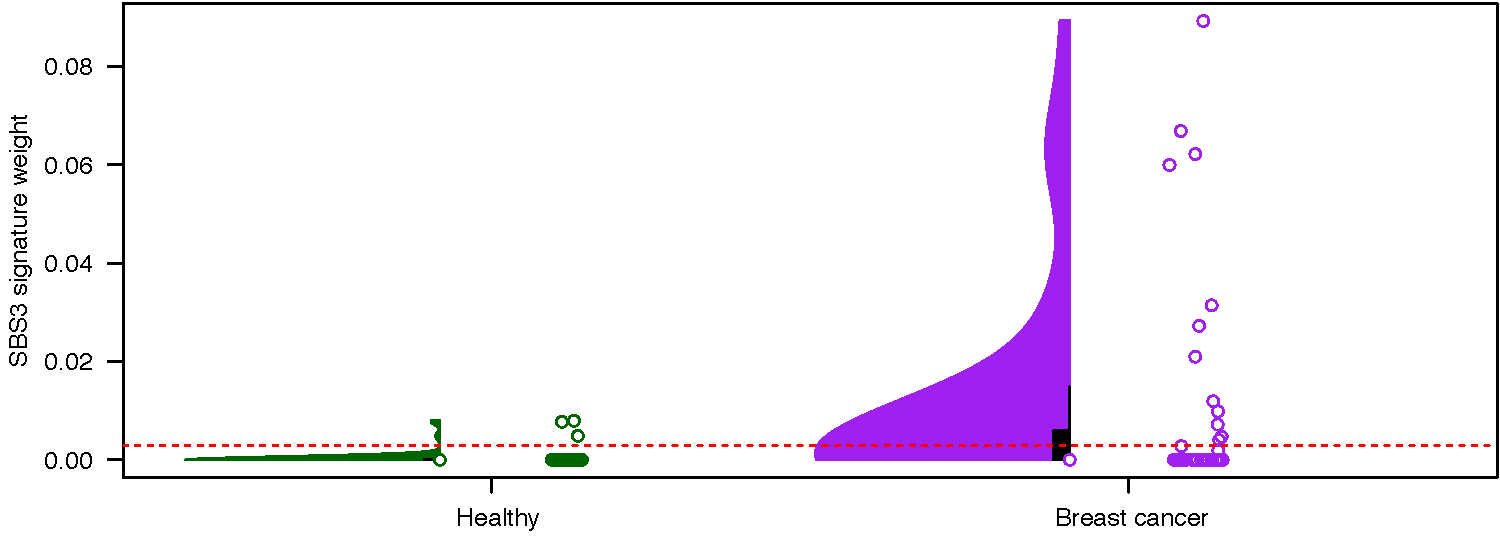
\includegraphics[width=.99\linewidth]{Figures/MisMatchFinder/SBS3Distributions.pdf}
\caption[SBS3 signature weight distribution in healthy and breast cancer samples]{SBS3 signature weight distribution in healthy and breast cancer samples: MisMatchFinder reported signature weights are shown as both a violinplot with boxplot in black and mean shown as white point on the left and the real measurements on the right; red line depicts classification cut-off twice at 0.003}\label{fig:mmf-SBS3distribution}
\end{figure}

With samples presenting with a SBS3 signature weight above 0.003 considered positive, we found 12 out of 39 (30\%) breast cancer samples and only misclassified 3 healthy samples as cancer positive. With only BRCA1/2 mutation positive cancers having a specific signature we only expected to be able to detect a subset of breast cancer patients. With homologous recombination deficiency (SBS3) being reported in up to to 40\% of breast cancers in previous studies \cite{AkashiTanaka2015}, our lower sensitivity for breast cancer could be caused by the lack of mutational signatures in the other 60\% of cases.

\section{Summary}
In this chapter we presented a new method to detect signatures from low coverage whole genome sequencing data as a complementary method to ichorCNA to detect and classify patient samples. Simulated data showed a high specificity of our method for deriving signatures. Real patient data confirmed that while there is a discrepancy between the current standard method of signature detection and MisMatchFinder, the most prevalent clinically relevant signatures were detected. Furthermore, MisMatchFinder was able to detect tumour presence in samples without additional input or need for matched normals.

As the concept has so far only been explored for SNVs, the method can be extended to also analyse DBS and even InDel signatures, which could potentially have an impact on the accuracy and sensitivity of the method.
And with more and more insight into the biological features of ctDNA additional enrichment steps, like fragment size selection, could be included to boost the signal of low tumour purity samples \cite{Mouliere2018,Markus2022}.

With some improvements and optimisations, MisMatchFinder could be seamlessly integrated into the ctDNA analysis workflows involving low coverage WGS to give insight into the mutational processes and resistance mechanisms \cite{Homburger2019,Chen2021}.
